\section{Presentation: Explanation of Methods}



\subsection{Overview of Workflow}




\subsection{NLP Methods}




\subsection{Keywords Co-Occurance Analysis}




\subsection{Keywords Graph Analysis}


\section{Results}

\begin{figure*}[t]
    \centering
    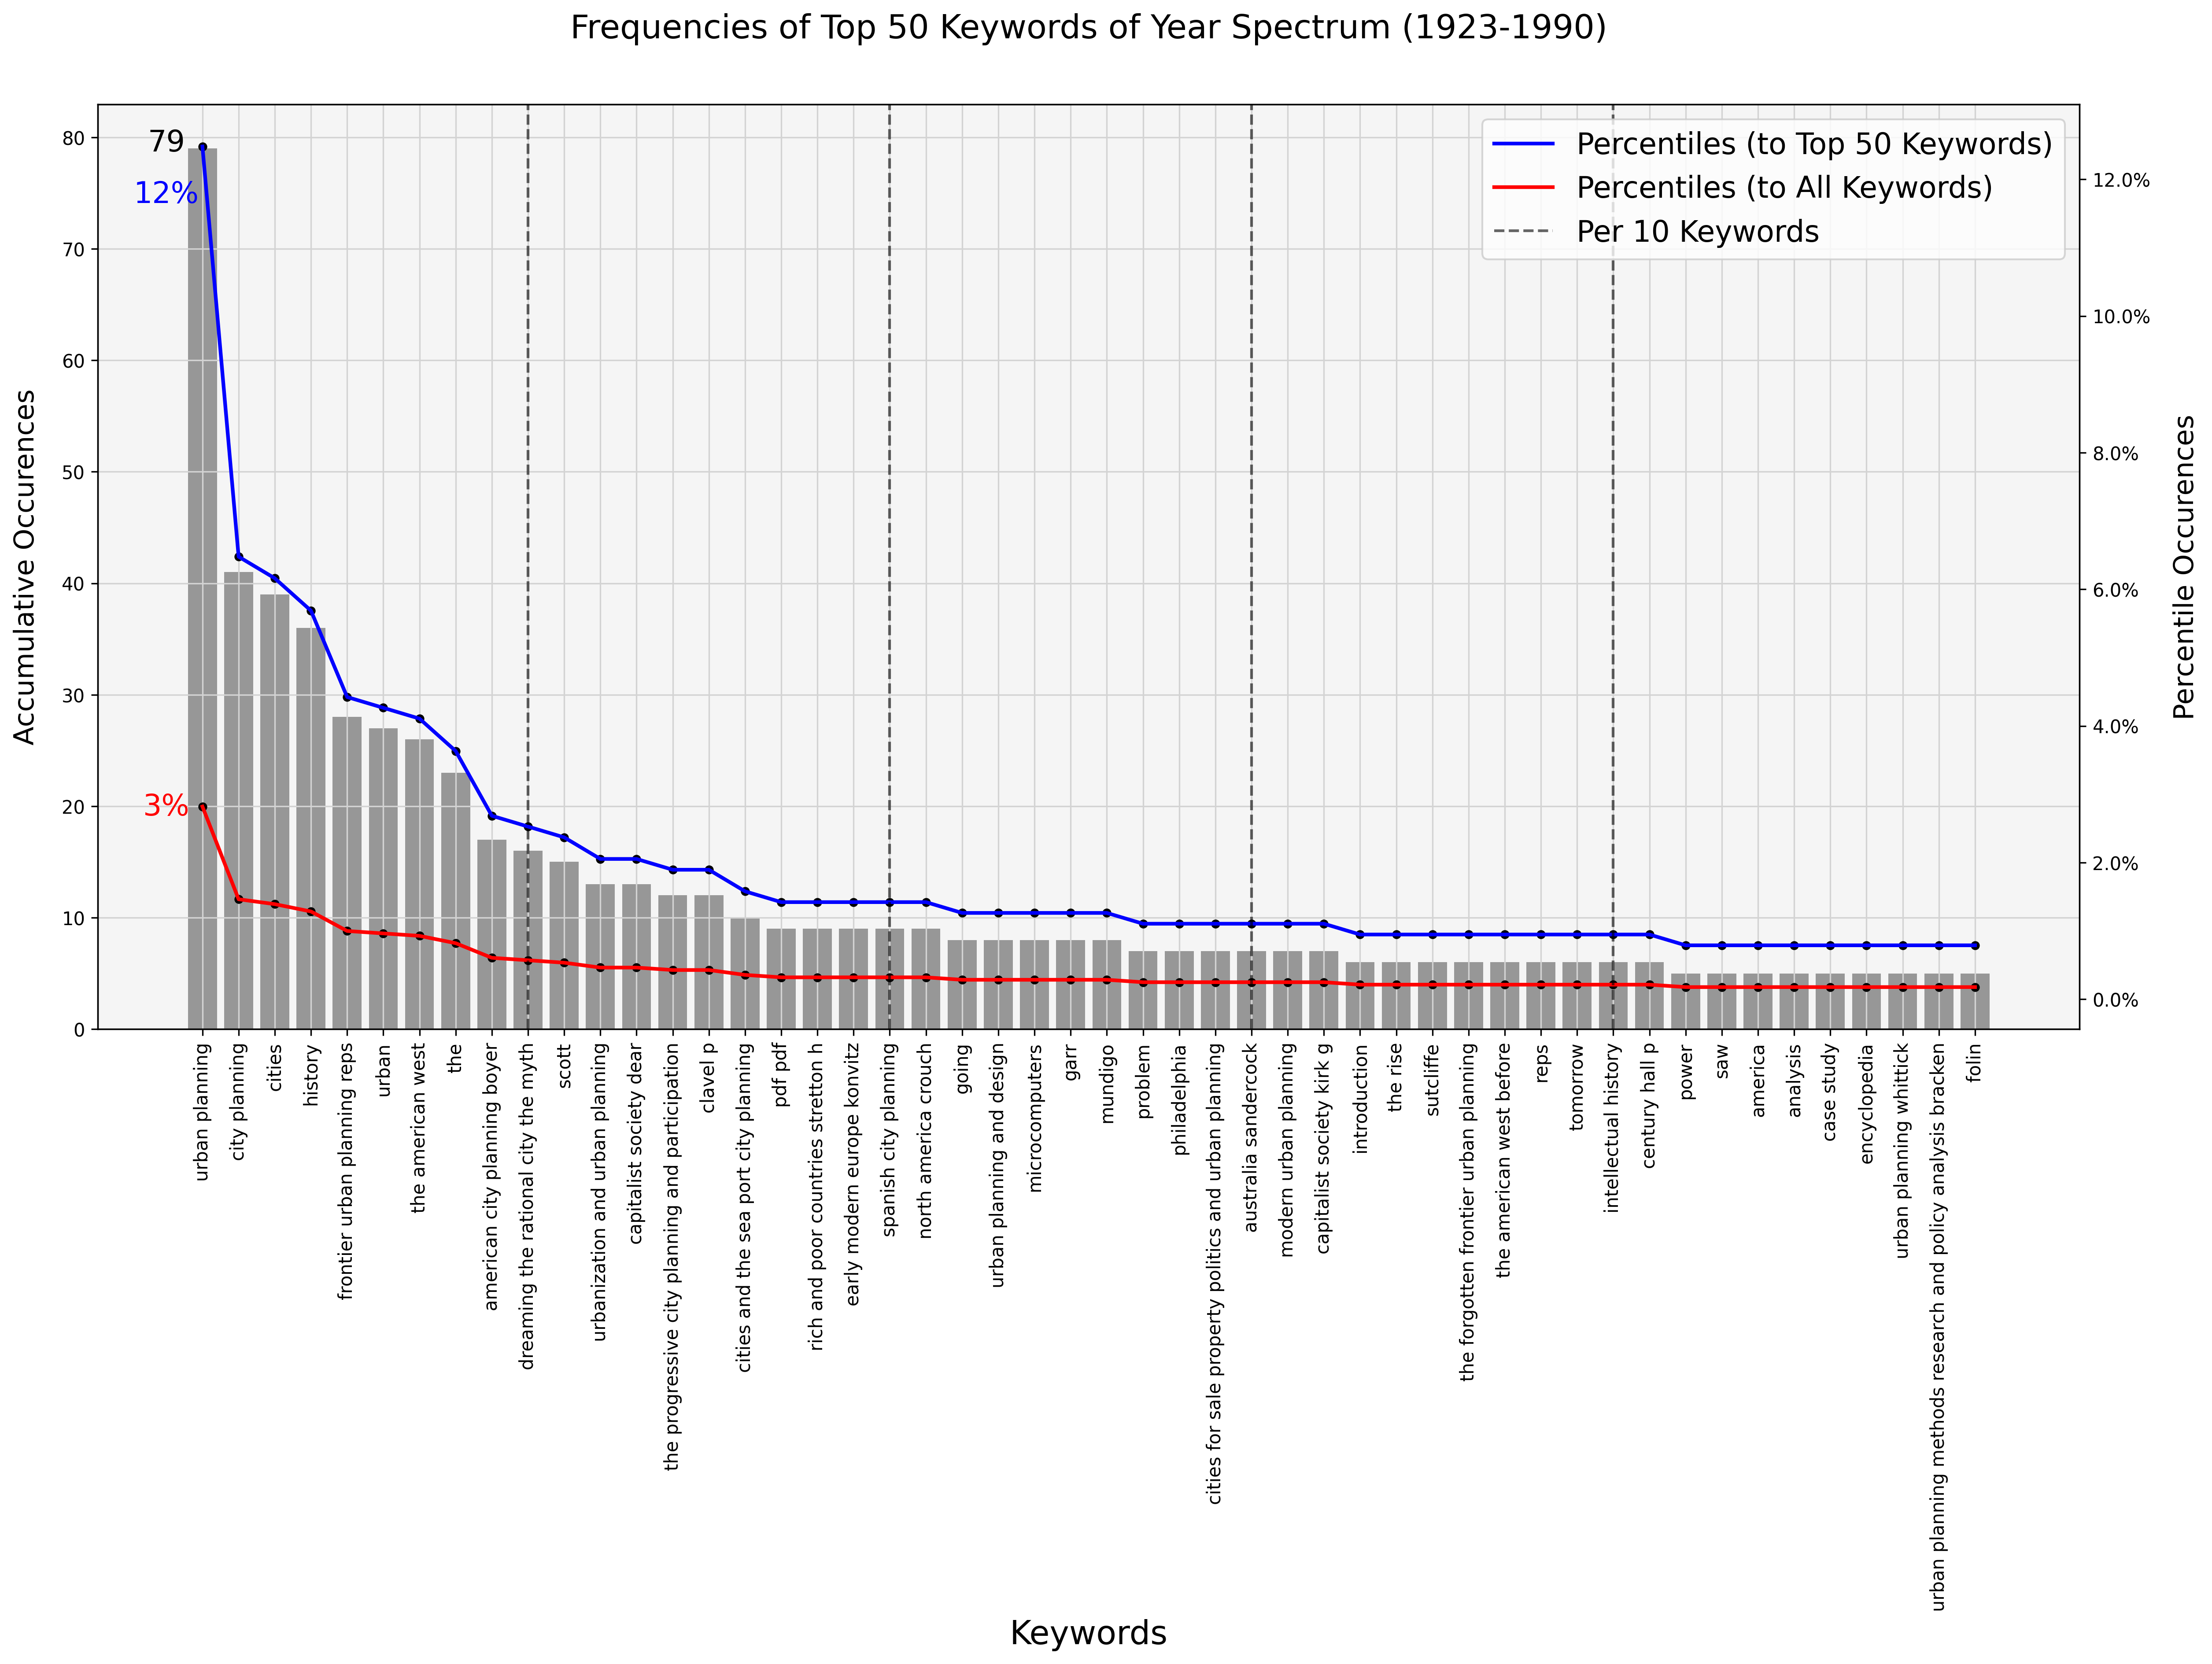
\includegraphics[width=0.98\textwidth]{./Outputs/All_year_single_word_frequencies.png}
    \caption{Macroscopic Fundamental Diagrams (MDFs) of Initial Plans (\textcolor{blue}{$\bullet$}) and Optimal Plans (\textcolor{red}{$\bullet$}), and Curves of Two-Regime Model (\textcolor{black}{\rule[0.2em]{1.5em}{0.15em}}) for All Tested Scenarios. Conditions with $qm$, $\alpha$ equals:(a)20$veh/h$,0.2. (b)20$veh/h$,0.4. (c)20$veh/h$,0.6. (d)20$veh/h$,0.8. (e)40$veh/h$,0.2. (f)40$veh/h$,0.4. (g)40$veh/h$,0.6. (h)40$veh/h$,0.8. (i)60$veh/h$,0.2. (j)60$veh/h$,0.4. (k)60$veh/h$,0.6. (l)60$veh/h$,0.8.}
    \label{fig:mdf_01}
    \end{figure*}